\documentclass[11pt]{article}
\usepackage[margin=1in]{geometry}
\usepackage{graphicx}
\usepackage{hyperref}
\usepackage{booktabs}
\usepackage{xcolor}
\usepackage{parskip}
\usepackage{enumitem}
\usepackage{fancyvrb}
\usepackage{caption}

\definecolor{ocean}{HTML}{1F6FB5}
\definecolor{sand}{HTML}{C9A66B}

\hypersetup{
  colorlinks=true,
  linkcolor=ocean!85!black,
  urlcolor=ocean!85!black,
  citecolor=ocean!85!black
}

\title{\textcolor{ocean}{\Huge Geomorphological Experiments for Amelia Island}\\[8pt]
\large An interactive simulation of barrier-island formation,\\
Holocene accretion, and Pleistocene welding}
\author{Paul Fishwick and Claude Code}
\date{May 2026}

\begin{document}
\maketitle

\begin{abstract}
\noindent
Amelia Island is a barrier island on the northeastern coast of Florida, at the southern
end of the Georgia Bight. It exhibits the classic ``double island'' structure of the
Bight: an older Pleistocene core (Silver Bluff terrace, $\sim$125\,ka) overlain on its
seaward side by a Holocene wedge that welded onto the core $\sim$5{,}000 years ago,
trapping the salt marsh now known as Egans Creek between them. Since welding, the
Atlantic face has prograded seaward, preserving a set of nested beach ridges most
clearly visible at Fort Clinch State Park on the island's north end. This document
specifies a set of computational experiments---an interactive web simulation, paired
with browser-driven verification---that reconstruct the island's coastline through
time. We ground the simulation in published sea-level data for northeastern Florida
\cite{hawkes2016}, in the formation theories of de Beaumont, Gilbert, McGee, and
Hoyt \cite{hoyt1967}, and in the narrative provided in lectures by the
Conserve Nassau organization \cite{cn_hopf,cn_dunes1,cn_dunes2}.
\end{abstract}

\tableofcontents
\newpage

\section{Motivation}

The question that motivated this work is direct: \emph{how did Amelia Island grow
into its present shape, and can that growth be made visible?}

The geomorphic story of the island is well established but is rarely shown as a
process. Most published material is text-and-diagram. A barrier island, however, is
a moving system: sea level oscillates by hundreds of feet over glacial cycles,
shorelines migrate tens of miles, and a sandbar a few miles offshore approaches the
mainland over millennia and finally welds onto it. These are kinematic phenomena
that benefit from a kinematic representation.

We propose a browser-based simulation in which the user drags a slider through
$\sim$125{,}000 years of coastline change and sees the island form. The simulation
is anchored on real geospatial data (modern shoreline from OpenStreetMap, terrain
signatures from USGS digital elevation models) and on real sea-level curves
\cite{hawkes2016,engelhart2012,toscano2003}.

\section{Geomorphic background}

\subsection{Barrier islands as a class of landform}

A barrier island is a long, narrow accumulation of sand parallel to a mainland coast,
separated from it by a lagoon, estuary, or marsh. Three classical theories have been
offered for how such islands form:

\begin{itemize}[leftmargin=2em]
\item \textbf{De Beaumont} (1845): offshore submarine bars built by shoaling waves
emerge above sea level. Flume experiments later showed bars cannot grow above
sea level by this mechanism alone, so this theory is now considered a partial
contributor.

\item \textbf{Gilbert} (1885, ``spit-accretion''): longshore drift builds a sandy spit
attached to the mainland; storms breach the spit, isolating an island. This
mechanism is observed in some modern systems.

\item \textbf{McGee} (1890, ``submergence''): rising sea level drowns mainland beach
ridges and dune fields, isolating them as islands with a new lagoon behind. Hoyt
(1967, \cite{hoyt1967}) supported this view with stratigraphic evidence---
specifically, the absence of shoreface sediment below early barriers, which would
be expected if the bars had emerged from below.
\end{itemize}

Modern process-based work \cite{mariotti2021} treats these as endmembers of a
self-organizing system whose behavior depends on three controls: the rate of
relative sea-level rise (RSLR), the supply of sand, and the back-barrier
accommodation space.

\subsection{Two regimes: transgressive and regressive}

Once formed, a barrier can be in one of two regimes (Table~\ref{tab:regimes}).

\begin{table}[h]
\centering
\caption{The two regimes of a barrier island, after \cite{mariotti2021}.}
\label{tab:regimes}
\begin{tabular}{p{3.5cm} p{5.5cm} p{5cm}}
\toprule
\textbf{Regime} & \textbf{Drivers} & \textbf{Signature} \\
\midrule
Transgressive (``rollover'') &
RSLR high, or sediment-starved; overwash moves sand landward across the island &
Washover fans on lagoon side; landward-migrating shoreline; ridges not preserved \\
\addlinespace
Regressive (``progradational'') &
Sediment supply exceeds accommodation; new sand builds seaward of older shoreline &
Beach-ridge plain (the nested arcs at Fort Clinch); seaward-younging \\
\bottomrule
\end{tabular}
\end{table}

Modeling \cite{mariotti2021} identifies a critical threshold near 2--5\,mm/yr RSLR:
above it, barriers are typically transgressive; below it, they can stabilize and
prograde. This threshold is consequential for Amelia.

\subsection{From sandbar to vegetated barrier}

A barrier island begins as a bare sandbar---a submerged or intertidal
accumulation of sediment where waves can no longer transport sand further
offshore. The transition to a stable, above-sea-level barrier requires
vegetation. The sequence is roughly:

\begin{enumerate}[leftmargin=2em]
\item \textbf{Submerged bar}: sediment accumulating offshore, below mean low
water.
\item \textbf{Emergent intertidal sandbar}: highest crests exposed at low
tide, bare or sparsely colonized by salt-tolerant pioneers (\emph{Uniola
paniculata}, \emph{Spartina patens}).
\item \textbf{Vegetated barrier}: dune grasses slow the wind, trap windblown
sand, and build foredunes. The foredunes shelter back-dune shrubs, and the
shrubs in turn shelter trees.
\item \textbf{Mature barrier with maritime forest}: oaks, palmettos, and a
closed canopy on stabilized terrain.
\end{enumerate}

The vegetation feedback is load-bearing for the system. Without plants, a
bare sandbar cannot retain sand against wind erosion, and it disperses. The
older Pleistocene core of Amelia exhibits the mature end of this sequence:
100{,}000 years of subaerial exposure has produced deep soils, rounded
slopes, and a maritime oak hammock. The younger Holocene wedge, by contrast,
shows steeper slopes, less mature soils, and a less stratified plant
community---it has had only 5{,}000 years above sea level.

For our reconstruction, the implication is that the offshore Holocene
sandbar between 8\,ka and 5\,ka was likely bare or sparsely vegetated.
After welding, the established vegetation network of the older Pleistocene
island could spread laterally onto the new wedge, accelerating its
stabilization.

\subsection{Pioneer-plant species and the binding mechanism}

Hopf's lectures \cite{cn_hopf_videoreport} identify the specific plant
species responsible for binding the loose quartz sand of Amelia's dunes:

\begin{itemize}[leftmargin=2em]
\item \textbf{Sea oats} (\emph{Uniola paniculata}) --- the most critical
pioneer species. Highly salt-tolerant, thrives when partially buried by
windblown sand, and possesses a fibrous root network extending up to
$\sim$30 feet deep. These roots physically bind the loose quartz grains,
turning a passive sand pile into a stable foredune.
\item \textbf{Bitter panicgrass} (\emph{Panicum amarum}) --- ground cover
that traps sand at lower elevations and stabilizes the dune face.
\item \textbf{Railroad vine} (\emph{Ipomoea pes-caprae}) --- a creeping
vine that spreads across bare sand surfaces, slowing wind and trapping
the next increment of windblown grains.
\end{itemize}

\noindent When this vegetation is destroyed---by foot traffic, vehicle
crossings, or storm overwash---a bowl-shaped depression called a
\emph{blowout} forms. Blowouts are conduits: during the next storm
surge, seawater penetrates the island through them, eroding back-dune
areas that would otherwise have been protected.

\subsection{Soil pedology: Pleistocene Spodosols vs.\ Holocene Entisols}

The age difference between the Pleistocene core and the Holocene wedge
is recorded not only in topography but also in \emph{soil maturity}.
The video report \cite{cn_hopf_videoreport} synthesizes Hopf's discussion
of the two distinct soil profiles:

\begin{itemize}[leftmargin=2em]
\item \textbf{Pleistocene core} ($\sim$125\,ka): Mature \textbf{Spodosols}.
After $\sim$100{,}000 years of subaerial exposure, organic acids from
decomposing leaf litter have leached down through the upper sand layers,
mobilizing iron and aluminum oxides. These re-precipitate at depth as a
dark, cemented \textbf{Bh (spodic) horizon}---a coffee-grounds-colored
band visible in soil pits in the Fernandina downtown and Plantation
areas. The presence of this horizon is diagnostic of long subaerial
exposure and reduced drainage; it is also responsible for the acidic
pH and the live-oak/Southern-magnolia maritime hammock vegetation.
\item \textbf{Holocene wedge} ($\sim$5\,ka and younger): \textbf{Entisols}---
unconsolidated, young, active sands with essentially no horizon
development. Color is light tan to white (high quartz, modest shell
content). The plant community is the early-successional dune complex
described above: sea oats, panicgrass, sea grape, saw palmetto.
\end{itemize}

\noindent This pedological contrast is independent confirmation of the
double-island age structure. Two adjacent surfaces with such different
soils cannot have weathered together; they were exposed at different
times. The Bh horizon is essentially a slow geologic clock that has
been ticking on the Pleistocene side for $\sim$100\,kyr longer than on
the Holocene side.

\subsection{The transgressive sandbar---what it looks like}

The offshore Holocene sandbar that approaches Amelia between $\sim$8\,ka
and $\sim$5\,ka deserves its own treatment, because it is geomorphically
the most interesting (and visually the most distinctive) feature in the
animation. It is a \emph{proto-barrier island}: a long, narrow ridge of
sand parallel to the existing shoreline, separated from the mainland by
a developing lagoon, intermittently emergent at low tide.

\paragraph{Modern analogs.}
Many present-day barrier islands look exactly like Amelia's offshore
sandbar did at 8--5\,ka:

\begin{itemize}[leftmargin=2em]
\item \textbf{Outer Banks, North Carolina} ($\sim$320\,km long, 0.5--3\,km
wide) --- the textbook transgressive barrier, still migrating landward.
\item \textbf{Padre Island, Texas} ($\sim$182\,km long, 0.5--5\,km wide)
--- the longest barrier island in the world; same long-narrow geometry.
\item \textbf{Fire Island, New York} ($\sim$50\,km long, $\sim$0.5\,km
wide) --- another active transgressive barrier.
\item \textbf{Cumberland Island, Georgia}, immediately north of Amelia
--- the same Georgia Bight ``double island'' as Amelia, just slightly
older. The Holocene wedge welded onto its Pleistocene core in the same
process described here.
\end{itemize}

\paragraph{Why long and narrow.}
The form arises from three balanced controls:

\begin{itemize}[leftmargin=2em]
\item \textbf{Length} is set by along-shore continuity of sediment supply.
Longshore drift moves sand parallel to the coast and accumulates it into
a continuous ridge wherever sediment supply is positive. For Amelia's
ancestor bar, the supply came primarily from the St.\ Marys River and from
sand reworked across Cumberland Sound.
\item \textbf{Width} is constrained by the equilibrium between wave erosion
on the seaward face and sand-supply deposition. During the active
transgressive phase, this equilibrium width is typically 100--500\,m;
modern transgressive barriers stay at this scale until sea-level rise
slows enough for them to stabilize and widen.
\item \textbf{Curvature} mirrors the existing shoreface. The bar forms
parallel to whatever coastline already exists, so its plan-view shape
follows the curve of Amelia's modern Atlantic shore (which is, in turn,
inherited from the Pleistocene core's geometry).
\end{itemize}

\paragraph{The landward migration.}
While sea level rose rapidly (rates above $\sim$5\,mm/yr), the bar could
not stabilize at any fixed offshore position. Storm overwash carried sand
from the seaward face across the bar to the lagoon side, depositing it as
washover fans. Over centuries, this net landward sand transport---combined
with continued retreat of the equilibrium profile---caused the entire bar
to ``roll over'' shoreward. Estimated migration rate during the slowing-
RSLR mid-Holocene is approximately 1\,km per millennium, consistent with
Frank Hopf's reference statement that the bar ``started out about four or
five miles out from where we are today on the coastline'' at $\sim$8\,ka
\cite{cn_dunes1}.

\paragraph{Visualization choices.}
In the simulation, the bar appears as a pale dashed polygon east of
Amelia, in two discrete snapshots (8\,ka and 6\,ka). Several
simplifications apply:

\begin{itemize}[leftmargin=2em]
\item \textbf{The dashed outline} signals that the bar is an inferred,
migrating feature rather than a fixed landform with a known boundary.
\item \textbf{Width} is rendered at $\sim$300\,m for visibility; real
transgressive bars were probably 50--200\,m wide at this stage and
widening as they slowed.
\item \textbf{Only the emergent crest} is shown; in reality the bar has
a submerged base extending 1--3\,km further seaward at depth.
\item \textbf{Migration} is rendered as two discrete positions rather
than a continuous motion---a fidelity-vs-clarity tradeoff. The
intermediate position is implicit; the user reading the slider can
mentally interpolate.
\end{itemize}

After welding at $\sim$5\,ka, the bar polygon disappears from the
animation and the Holocene wedge polygon takes over as the bar's
permanent successor on the welded island.

\subsection{Beach ridges at Fort Clinch---what Hopf describes
vs.\ what we infer}

The progradational ridge complex at Fort Clinch State Park appears in
the simulation as a sequence of nested arcs accreting eastward from
$\sim$5\,ka to the present. The ridges are real and visible on USGS
topographic maps and satellite imagery, but the doc needs to be clear
about which parts of the model derive from Hopf's lectures and which
parts are inferred from the broader literature.

\paragraph{What Hopf describes explicitly.}
Hopf discusses the \emph{post-jetty} ridges---the outermost subset of
the ridge complex, formed between 1881 and today as a direct
consequence of the St.\ Marys Entrance jetty construction. In
\emph{Dunes Pt 1} he says \cite{cn_dunes1}:

\begin{quote}
\itshape
``\ldots up against the state park boundary, and you can see our
Holocene dune over there against the park, nice high dune, protective.
And then this series of dune ridges that grew up after they put in the
jetty---and then in front of that is the rock revetment built by the
Corps of Engineers after Hurricane Dora hit in 1964\ldots''
\end{quote}

\noindent and in \emph{Dunes Pt 2} \cite{cn_dunes2}:

\begin{quote}
\itshape
``\ldots the sand that would go in like on the flood tide sort of got
trapped there, and that's how that little piece of brand new land got
formed on the north end of the island\ldots and there's a bunch of
little dune ridges up on the island there up on that section.''
\end{quote}

Hopf attributes the post-jetty ridges specifically to flood-tide sand
being trapped against the south jetty after 1881. He confirms their
location at the north end of Amelia (Fort Clinch State Park) and
distinguishes them from the older, higher Holocene dune inland.

\paragraph{What is inferred from the literature.}
Hopf does \emph{not} enumerate the older, \emph{pre-jetty} ridges
individually. The seven older ridges in our model (ages 5\,ka, 4\,ka,
3\,ka, 2\,ka, 1\,ka, 500\,yr BP, and pre-jetty 1880 CE) are inferred
from OSL-dated comparable Florida barrier systems:

\begin{itemize}[leftmargin=2em]
\item Rink and Forrest \cite{rink2008} dated Cape Canaveral and Merritt
Island beach ridges with quartz OSL, deriving an average accretion
rate of $\sim$80 years per ridge and $\sim$135\,m of seaward land
accretion per century.
\item Forrest et al.\ \cite{forrest2007} dated the St.\ Vincent Island
strandplain (Florida Panhandle) with OSL, getting inter-ridge intervals
of 78--148 years for the younger ridges.
\end{itemize}

\noindent Applied to Amelia's $\sim$5{,}000-year post-welding
progradation, those rates predict 30--60 ridges \emph{if} ridge
formation were continuous. In practice, only $\sim$8--15 major arcs
are preserved at Fort Clinch (storm-deposited foredunes, not annual
ones, and many smaller ridges presumably eroded or amalgamated). Our
model renders eight, consistent with the major-arc count visible in
satellite imagery and the USGS topographic map referenced in
Hopf's lectures.

\paragraph{Bottom line.}
The ridge complex's existence and overall pattern is Hopf's; the
specific per-ridge ages are interpolated from comparable Florida
systems. We label individual ridges by their inferred ages but
acknowledge the dating is by analogy, not direct OSL on Amelia.

\subsection{The Georgia Bight ``double island'' pattern}

Along the Atlantic coast of Georgia and northeastern Florida, the Holocene barrier
islands did not form on a virgin shelf. They formed offshore of an older set of
Pleistocene barriers that had survived as elevated remnants. As sea level rose
through the Holocene, the offshore Holocene bars migrated landward and \emph{welded}
onto the Pleistocene cores. Hoyt and Hails \cite{hoyt1967} identified six major
Pleistocene shoreline complexes in coastal Georgia, each a former barrier-lagoon
system, now overlain on its seaward side by a Holocene wedge. This pattern produces
the double-island islands of the Bight: Hilton Head, Tybee, Wassaw, Ossabaw, St.
Catherines, Sapelo, the St. Simons group, Jekyll, Cumberland, and Amelia at the
southern end \cite{georgiabight}.

\subsection{Amelia in Hayes' Georgia Bight classification}

Hayes' comprehensive Georgia Bight chapter \cite{georgiabight} divides the bight
into six along-shore \emph{compartments}, each with a distinctive shoreline
character. Amelia Island sits in \textbf{Compartment V} (St.\ Simons Sound to
the St.\ Johns River mouth), which Hayes calls the
\textbf{``Combo-Drumstick Region.''} The compartment contains just three large
drumstick-shaped islands: \textbf{Jekyll, Cumberland, and Amelia}. Hayes writes
\cite{georgiabight}:

\begin{quote}
\itshape
``Each of the islands has a core of Pleistocene barrier-island sand with welded
Holocene beach ridges usually attached to the northern and southern ends.''
\end{quote}

\noindent This is the exact structure the simulation renders: a Pleistocene
core with Holocene wedge welded onto its eastern face, and the most prominent
beach-ridge complex preserved at the \emph{north} end (Fort Clinch State Park).
Three further Hayes findings inform the simulation:

\begin{itemize}[leftmargin=2em]

\item \textbf{Mixed-energy ``drumstick'' morphology.} Drumstick-shaped islands
are characteristic of mixed-energy, mesotidal coasts---those with tidal range
2--4\,m and moderate wave energy. The drumstick form arises from updrift
sediment trapping by ebb-tidal deltas, producing an asymmetric island with a
broad northern bulge (the ``thigh''). Amelia displays this geometry; the Fort
Clinch ridge complex is its northern bulge.

\item \textbf{Compartment composition.} Compartment V's outer shoreline is
68\% regressive mixed-energy barrier islands (the Holocene beach-ridge
sections), 19\% eroding Pleistocene island core, and 13\% harbor/sound
entrances. The 19\% \emph{eroding} Pleistocene cores is a useful reality
check: the Pleistocene face is not stable. Amelia's western (Amelia River)
side is subject to slow erosion from estuarine and tidal currents.

\item \textbf{Narrow back-barriers from the Ocala Uplift.} Hayes attributes
the narrow back-barrier regions of Compartment V's islands to the tectonic
influence of the \textbf{Ocala Uplift}, a regional structural high that
shoals the inner shelf. This same uplift explains why Amelia's Pleistocene
core sits relatively close to today's mainland (the marsh between Amelia and
the mainland is narrow compared to, say, the broader Mississippi Sound
behind the Mississippi--Alabama barriers).

\end{itemize}

\subsection{Sediment supply: a coastal-plain (``blackwater'') river}

A subtle but important point in Hayes \cite{georgiabight} is that the St.\
Marys River---Amelia's principal sand source from the north---is a
\emph{coastal-plain} or \emph{blackwater} river, not a piedmont river. Its
drainage basin lies entirely within the coastal plain (it does not reach the
Appalachian foothills). Hayes notes that coastal-plain rivers ``presently
deliver only second-cycle, reworked sediments to the shoreline.'' Amelia's
Holocene beach-ridge sand is therefore \emph{recycled Pleistocene sand}, not
fresh first-cycle sediment from the mountains---a detail worth keeping in
mind when reasoning about long-term sediment budgets and the post-jetty
sand-starvation problem that Frank Hopf describes (the jetty intercepts
this already-limited recycled-sand supply, accelerating central-Amelia
beach erosion until the modern Nassau County Shore Protection Project
began artificially restoring it).

\paragraph{Mineralogical signature.}
Beyond the bulk quartz, Hopf \cite{cn_hopf_videoreport} identifies the
heavy-mineral fingerprint of Amelia's sand as a marker of its ultimate
Appalachian provenance: \textbf{zircon}, \textbf{staurolite}, and
\textbf{tourmaline}---all metamorphic accessory minerals diagnostic of
high-grade-metamorphic source rocks in the Appalachian--Piedmont
hinterland. These minerals were eroded out of the mountains over
$10^8$ years and survived multiple cycles of transport and deposition
because they are mechanically and chemically very resistant. Even
though the St.\ Marys delivers reworked sand today, the original
provenance signature is preserved. Frank Hopf also notes a high
\textbf{titanium-oxide} content (the dark heavy-mineral fraction
visible as the ``black sand'' streaks on Amelia's beach at low tide)
that was once considered for commercial mining---an extraction that
fortunately did not proceed at Amelia (though it did at Ponte Vedra
to the south, where the resulting beach erosion is still felt).

\subsection{Florida marine terraces}

The Pleistocene core of Amelia sits on the Silver Bluff terrace, formed during the
Sangamonian interglacial (Marine Isotope Stage 5e) when sea level stood
$\sim$6\,m above present \cite{georgyofflorida}. Florida exposes a sequence of older
terraces stepping up in elevation and back in age: Pamlico, Talbot, Penholoway, and
Wicomico. Only the Silver Bluff terrace is relevant to Amelia.

\section{Sea-level history used in the simulation}

The most directly relevant sea-level reconstruction for Amelia is Hawkes et al.\
\cite{hawkes2016}, which produced 25 sea-level index points spanning 8.0\,ka to
2.0\,ka from salt-marsh foraminifera at sites in northeastern Florida. Three
findings from that work shape the simulation:

\begin{enumerate}[leftmargin=2em]
\item Relative sea level rose $\sim$5.7\,m in northeastern Florida over the last
8.0\,ka.
\item There is \textbf{no Holocene highstand} at this latitude---the rise has been
monotonic. This contrasts with the central US Atlantic coast and the Caribbean,
which show mid-Holocene highstands.
\item The pattern reflects the collapse of the Laurentide Ice Sheet's proglacial
forebulge, which produces ongoing subsidence at this latitude.
\end{enumerate}

We extend the curve back to 125\,ka by combining \cite{hawkes2016} with the
Caribbean Holocene curve of Toscano and Macintyre \cite{toscano2003}, the
Engelhart and Horton US Atlantic database \cite{engelhart2012} for the mid-
Holocene tail, and Lambeck et al.\ for the Last Glacial Maximum lowstand. The
resulting target curve is summarized in Table~\ref{tab:sealevel}.

\begin{table}[h]
\centering
\caption{Sea-level snapshots used by the simulation. Negative values indicate sea
level below present. Sources are cited where each value is anchored.}
\label{tab:sealevel}
\begin{tabular}{rrl}
\toprule
\textbf{Years BP} & \textbf{RSL (m)} & \textbf{Phase / source} \\
\midrule
125{,}000 & $+6$ & Eemian (MIS 5e) highstand; Silver Bluff terrace \\
\phantom{1}80{,}000 & $-20$ & MIS 5a/4 transition \\
\phantom{1}20{,}000 & $-120$ & Last Glacial Maximum \\
\phantom{1}14{,}500 & $-90$ & onset of Meltwater Pulse 1A \\
\phantom{1}13{,}500 & $-72$ & end of MWP-1A ($\sim$18 m rise in 500 yr) \\
\phantom{11}8{,}000 & $-5.7$ & Hawkes et al.\ 2016 anchor \\
\phantom{11}5{,}000 & $-2.0$ & Welding event (slow RSLR, $\sim$1 mm/yr) \\
\phantom{11}2{,}000 & $-0.5$ & Late Holocene progradation \\
\phantom{1111}150 & $-0.2$ & Pre-jetty (1880 CE) \\
\phantom{11111}0 & $\phantom{-}0.0$ & Present (2026 CE) \\
\bottomrule
\end{tabular}
\end{table}

\section{Narrative arc of Amelia Island}

The reconstruction proceeds in six phases.

\paragraph{Phase 0: Pleistocene core forms ($\sim$125\,ka).}
During the Sangamonian highstand, sea level stood $\sim$6\,m above present and a
barrier island formed on the Silver Bluff terrace at the location of today's
western Amelia. Behind it: lagoon and salt marsh. The same system that produced
neighboring Cumberland Island.

\paragraph{Phase 1: Lowstand exposure (125--20\,ka).}
Sea level fell $\sim$125\,m through the Wisconsinan glaciation. The Pleistocene
Amelia stood as an inland hill, with the shoreline retreating to a Last Glacial
Maximum position roughly 130\,km east of today's coast, near the $-120$\,m
bathymetric contour on the continental shelf. During this $\sim$100{,}000 year
exposure, the Pleistocene sands matured: deeper soils formed, slopes rounded,
oak-hammock vegetation established.

\paragraph{Phase 2: Holocene transgression (20--8\,ka).}
As the Laurentide and Eurasian ice sheets retreated, sea level rose rapidly,
particularly during Meltwater Pulse 1A (14.7--13.5\,ka, $\sim$36\,mm/yr). RSLR
this fast keeps barriers in the transgressive regime: ephemeral sandbars formed,
drowned, and reformed at landward positions on the migrating shoreface. None
were preserved in their original locations.

\paragraph{Phase 3: The approach (8--5\,ka).}
By 8\,ka, sea level was within $\sim$6\,m of present and rising more slowly
($\sim$2--3\,mm/yr per \cite{hawkes2016}). A persistent Holocene sandbar formed
roughly four miles east of the Pleistocene core. The shallow water between the
sandbar and the older island became a protected lagoon. Mud---which will not
settle out of suspension on its own---accumulated as oysters and clams filtered
it from the water and deposited it as faecal pellets. Salt marsh built upward
on this biogenic mud. The future Egans Creek wetland began to form.

\paragraph{Phase 4: Welding ($\sim$5\,ka).}
RSLR slowed below the stabilization threshold ($\sim$2\,mm/yr). The Holocene
sandbar stopped retreating, grew vertically and laterally, and finally welded
onto the Pleistocene island---first at the south end of Amelia, then propagating
north. The Egans Creek marsh was sealed in between, becoming a relict back-barrier
lagoon. This is the most visually distinctive event in the simulation.

\paragraph{Phase 5: Progradation (5\,ka--1880 CE).}
With slow RSLR, abundant longshore sand from the St.\ Marys River to the north,
and the welded island as a fixed anchor, the Atlantic face of Amelia began to
build seaward. Successive shoreline positions are preserved as beach ridges,
each separated by 80--150 years on comparable Florida systems
\cite{rink2008,forrest2007}. At Fort Clinch on the north end, the curving plan
form of the island favored maximum accretion, producing the nested arc-shaped
ridges visible from the air and on USGS topography.

\paragraph{Phase 6: Human modification (1880--present).}
The St.\ Marys Entrance jetty, completed in 1881 and extended afterward,
intercepted the southbound longshore sand transport at the north end of Amelia.
The result was an additional fillet of accretion---the ``post-jetty dunes''
visible on the seaward side of the historical shoreline at Fort Clinch State
Park---superimposed on the natural pattern over 150 years rather than the
natural rate of 80--150\,years per ridge. The Nassau County Shore Protection
Project (USACE Jacksonville District, with Olsen Associates) now manages
periodic beach nourishment on the developed central portion of Amelia.

\section{Simulation design}

\subsection{Goal}
The simulation is a single-page web application. The user opens \texttt{index.html}
in a browser. A Leaflet \cite{leaflet} map centered on Amelia Island shows the
present-day coastline on an OpenStreetMap basemap. A horizontal slider, ranging
from 125\,ka BP to the present, is positioned below the map. Dragging the slider
re-renders the map with the polygons appropriate to that time slice: the
Pleistocene core (when above sea level), the Holocene wedge in its current state
(absent, offshore as a migrating bar, welded, or with progradational ridges), and
the salt marshes. A side panel displays a one-paragraph caption summarizing the
era, paraphrased from the source lectures and the published literature.

\subsection{Geometry}
Geometry is built from three sources:

\begin{enumerate}[leftmargin=2em]
\item \textbf{Modern island coastline}: queried from OpenStreetMap via the Overpass
API and exported to GeoJSON. This is real public-domain data.
\item \textbf{Pleistocene/Holocene boundary on the island}: traced once from the
USGS 3DEP digital elevation model. The Pleistocene core has the rounded, soil-
mature signature of an emerged terrace; the Holocene wedge has the corrugated
ridge-and-swale signature of progradational accretion. The boundary
approximately follows Egans Creek through the central island.
\item \textbf{Beach ridges at Fort Clinch}: digitized from satellite imagery and
DEM hillshade. We digitize 8 major ridges, consistent with the major arcs visible
in the field.
\end{enumerate}

Pre-welding paleo-coastlines (12\,ka, 8\,ka, 5\,ka) are reconstructed by offset
from the modern shoreline using the migration distances cited in the source
lectures (3--5 miles offshore at 12\,ka, approaching at $\sim$1\,mile per
millennium). These are labeled in the UI as interpretive reconstructions, not
measured paleoshorelines.

\subsection{Cross-section view}
A secondary panel renders the modern cross-section described by the source
lectures (Plantation, Little Nana, and Big Nana profiles): a young Holocene dune
on the Atlantic face, the Egans Creek marsh in the center, the older Pleistocene
core to the west, and the back-barrier marsh on the mainland side. The panel
animates the accretion of the cross-section through time, illustrating the
``two piles of sand on a bed of mud'' description Frank Hopf uses.

\subsection{Architecture}
\begin{itemize}[leftmargin=2em]
\item \texttt{index.html} --- single page, no build step.
\item \texttt{viewer.js} --- loads snapshot GeoJSONs, interpolates between them as
the slider moves, manages layer styling.
\item \texttt{style.css} --- Pleistocene shown in a muted earth-tone; Holocene
sand in a pale ridge-and-swale pattern; salt marsh in green; sea in blue.
\item \texttt{data/} --- one GeoJSON per snapshot, plus \texttt{sea\_level.json}.
\item \texttt{scripts/} --- Python utilities for data preparation and Selenium-
based verification.
\end{itemize}

\section{Verification with Selenium}

All HTML web tests are written in Selenium \cite{selenium}, per project standard.
The test suite (\texttt{tests/auto/test\_viewer.py}) launches a headless Chrome
browser, loads the application from a local HTTP server, waits for the Leaflet
map to fully initialize, and exercises the time slider through each defined
snapshot. For each snapshot, the test:

\begin{enumerate}[leftmargin=2em]
\item Sets the slider to the snapshot's target year.
\item Waits for the layer transition to complete and tiles to load.
\item Captures a full-page screenshot to \texttt{docs/fig/snapshot\_\textit{N}.png}.
\item Asserts that the expected layers are present in the DOM
(\texttt{.layer-pleistocene}, \texttt{.layer-holocene}, \texttt{.layer-marsh},
etc.\ as appropriate to the era).
\end{enumerate}

The same captured screenshots are referenced by this document via
\texttt{\textbackslash includegraphics}. The verification suite therefore serves
two roles: it tests the application, and it generates the figures embedded here.
This document is rebuilt by running the test suite, then \texttt{pdflatex} on
this file.

\section{User guide}

\subsection{Launching the simulation}

The simulation is a single static HTML file with no server-side dependencies.
From the project root, launch the bundled \texttt{start} script:

\begin{Verbatim}[fontsize=\small]
./start
\end{Verbatim}

The script checks whether port 8765 is already in use (and stops a stale
process if so), starts a local HTTP server, and opens
\texttt{http://localhost:8765/index.html} in the default browser. To stop
the server later:

\begin{Verbatim}[fontsize=\small]
./stop
\end{Verbatim}

\subsection{The map view}

On load, the application centers on Amelia Island at the present-day timestep.
The OpenStreetMap basemap shows the modern coastline, with the simulation's
geologic layers drawn on top: the Pleistocene core in muted earth tone, the
Holocene wedge in pale sand, the Egans Creek marsh in green, the Atlantic and
Amelia River in blue. Standard Leaflet pan and zoom controls are available; the
geologic layers re-render at every zoom level.

\subsection{The time slider}

A horizontal slider below the map ranges from 125{,}000\,years\,BP at the left
to the present (2026\,CE) at the right. Dragging the slider re-renders the
geologic layers to reflect the coastline at that time. The slider is
logarithmic in years\,BP, so most of its travel is in the Holocene, where the
welding event and beach-ridge progradation occur.

A play button below the slider animates the simulation forward from the current
position at one of three speeds (1$\times$, 5$\times$, 20$\times$). A reset
button returns the slider to 125\,ka.

\subsection{The era panel}

To the right of the map, an information panel updates as the slider moves. It
shows the current era name, the year\,BP, the relative sea level (in meters
versus today), and a one-paragraph caption describing what is happening at that
moment. Caption text is paraphrased from the source lectures
\cite{cn_hopf,cn_dunes1,cn_dunes2} and the published literature cited above.

\subsection{The cross-section panel}

A toggle in the upper-right opens a secondary panel showing the modern
cross-section of the island at the Plantation profile, after the cross-sections
in \cite{cn_hopf,cn_dunes1,cn_dunes2}. From west to east this shows: the Amelia River,
the mainland salt marsh, the Pleistocene core, the Egans Creek marsh, the
Holocene wedge with its beach ridges, the modern foredune, and the Atlantic
Ocean. As the time slider moves, the cross-section animates to show how each
component built up. The cross-section caption identifies the ``two piles of
sand on a bed of mud'' structure that Frank Hopf emphasizes.

\section{Results}

The figures below are captured directly by the Selenium suite as it exercises
the viewer through each defined snapshot. Each figure shows the full
application interface: the Leaflet map (left, top), the cross-section panel
(left, bottom), and the era panel (right) with current year, relative sea
level, and the narrative caption.

\begin{figure}[h!]
\centering
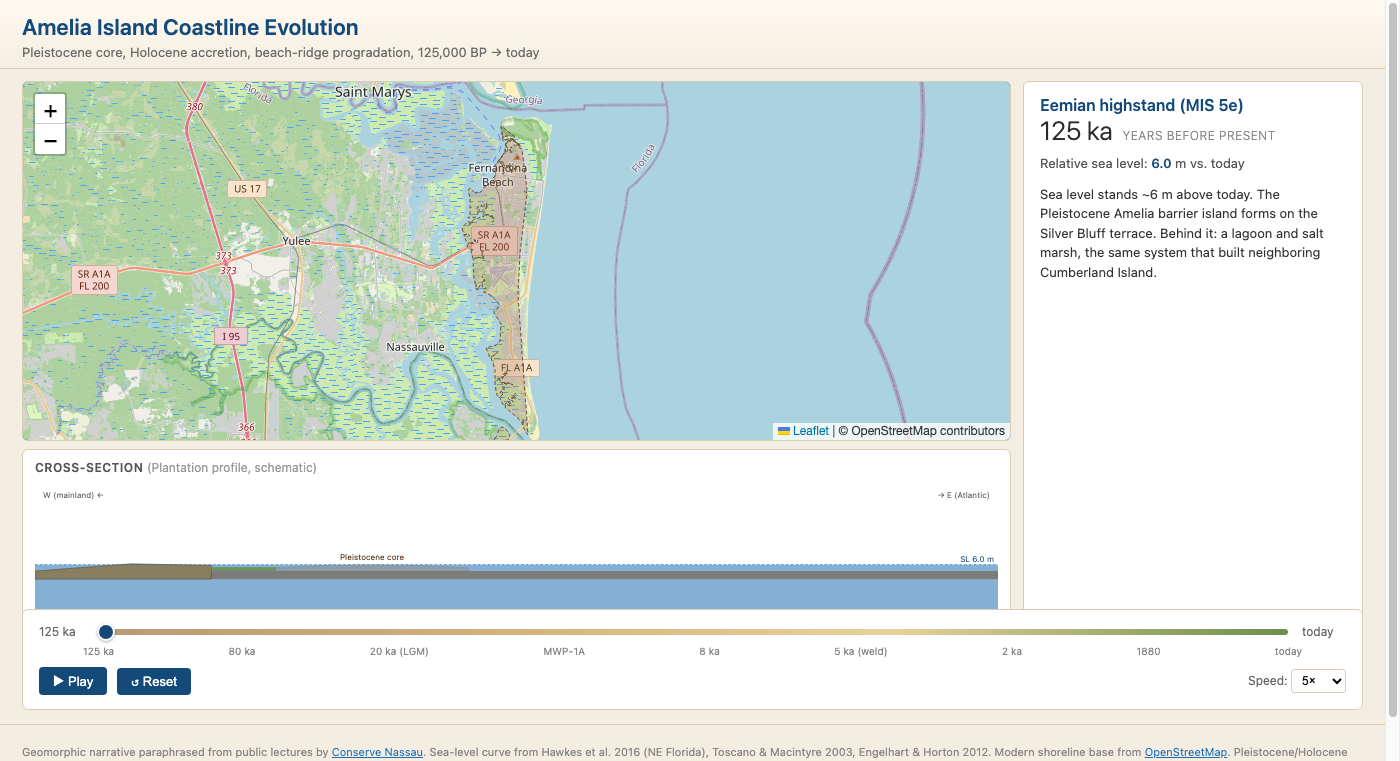
\includegraphics[width=0.95\textwidth]{fig/01_eemian_125ka.png}
\caption{Eemian highstand, 125\,ka. The Pleistocene core (Silver Bluff
terrace) is forming under a sea level $\sim$6\,m above today's. The cross-
section shows the future-Amelia footprint as a single body above the dashed
sea-level line; everything seaward of it will form later.}
\label{fig:eemian}
\end{figure}

\begin{figure}[h!]
\centering
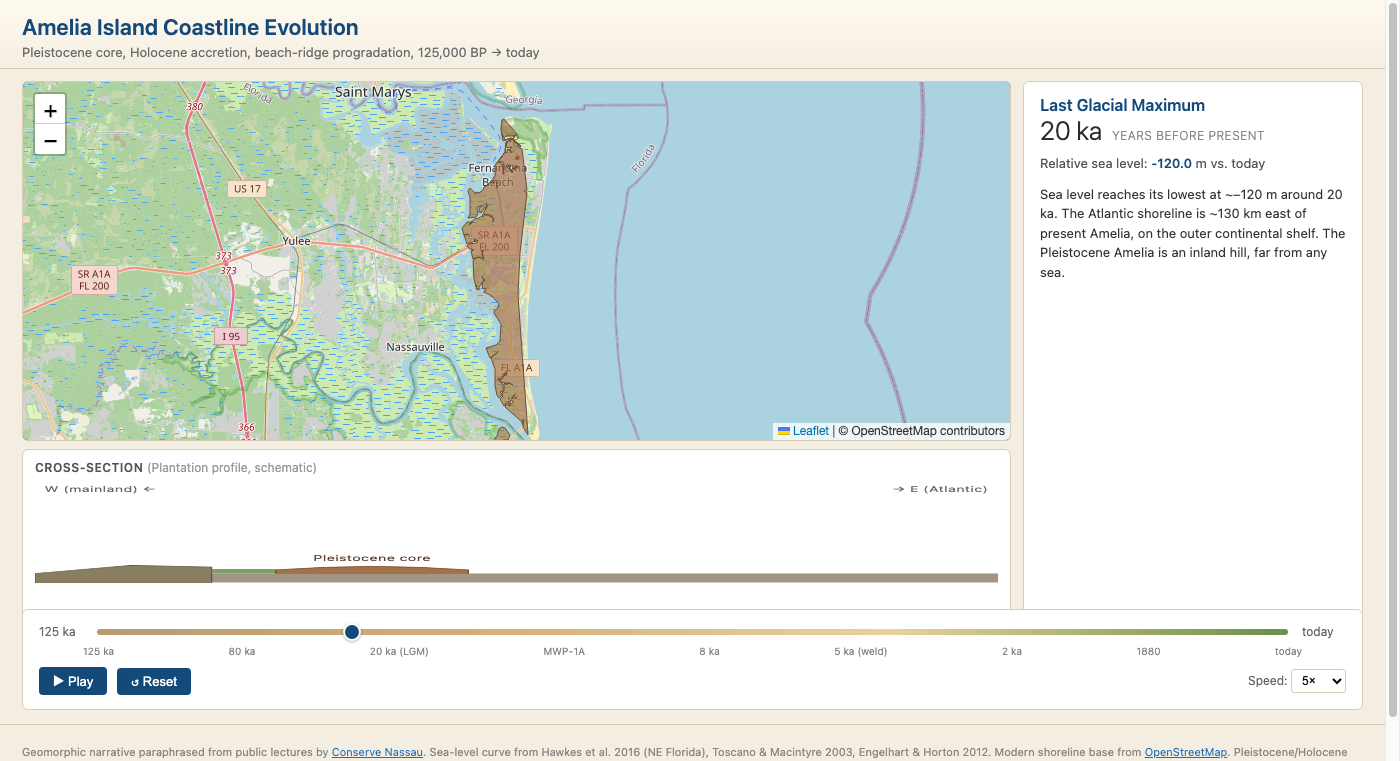
\includegraphics[width=0.95\textwidth]{fig/02_lgm_20ka.png}
\caption{Last Glacial Maximum, 20\,ka. Sea level $-120$\,m. The red dashed
hint line at the right edge of the map marks the LGM Atlantic shoreline
$\sim$130\,km east. The Pleistocene Amelia stands as an inland hill, far
from any coast.}
\label{fig:lgm}
\end{figure}

\begin{figure}[h!]
\centering
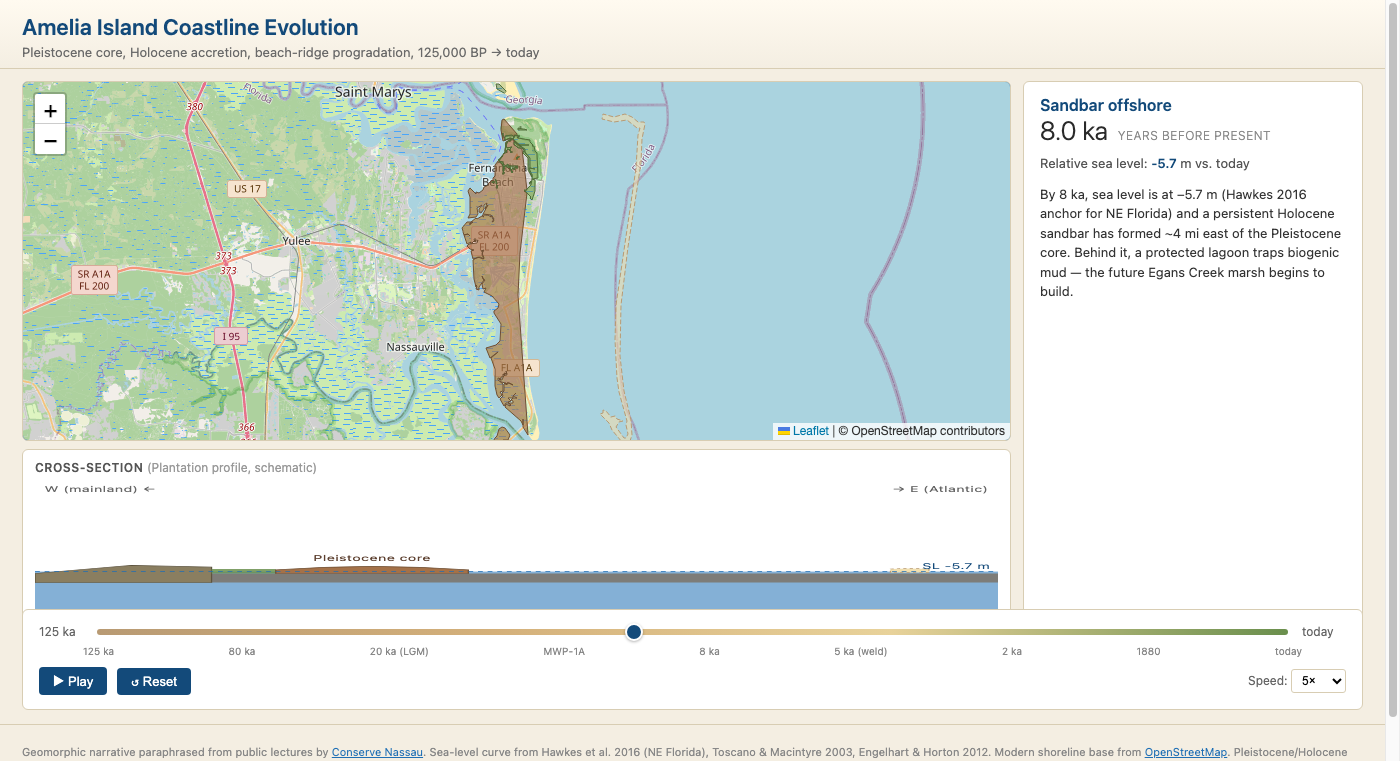
\includegraphics[width=0.95\textwidth]{fig/03_sandbar_8ka.png}
\caption{Holocene transgression, 8\,ka. Sea level $-5.7$\,m (Hawkes et al.\
2016 anchor). A persistent Holocene sandbar (pale dashed polygon to the east
of the island) has formed $\sim$4\,mi east of the Pleistocene core. In the
cross-section: the bar appears offshore (right), and the Egans Creek marsh
begins to fill the lagoon between bar and core.}
\label{fig:sandbar8ka}
\end{figure}

\begin{figure}[h!]
\centering
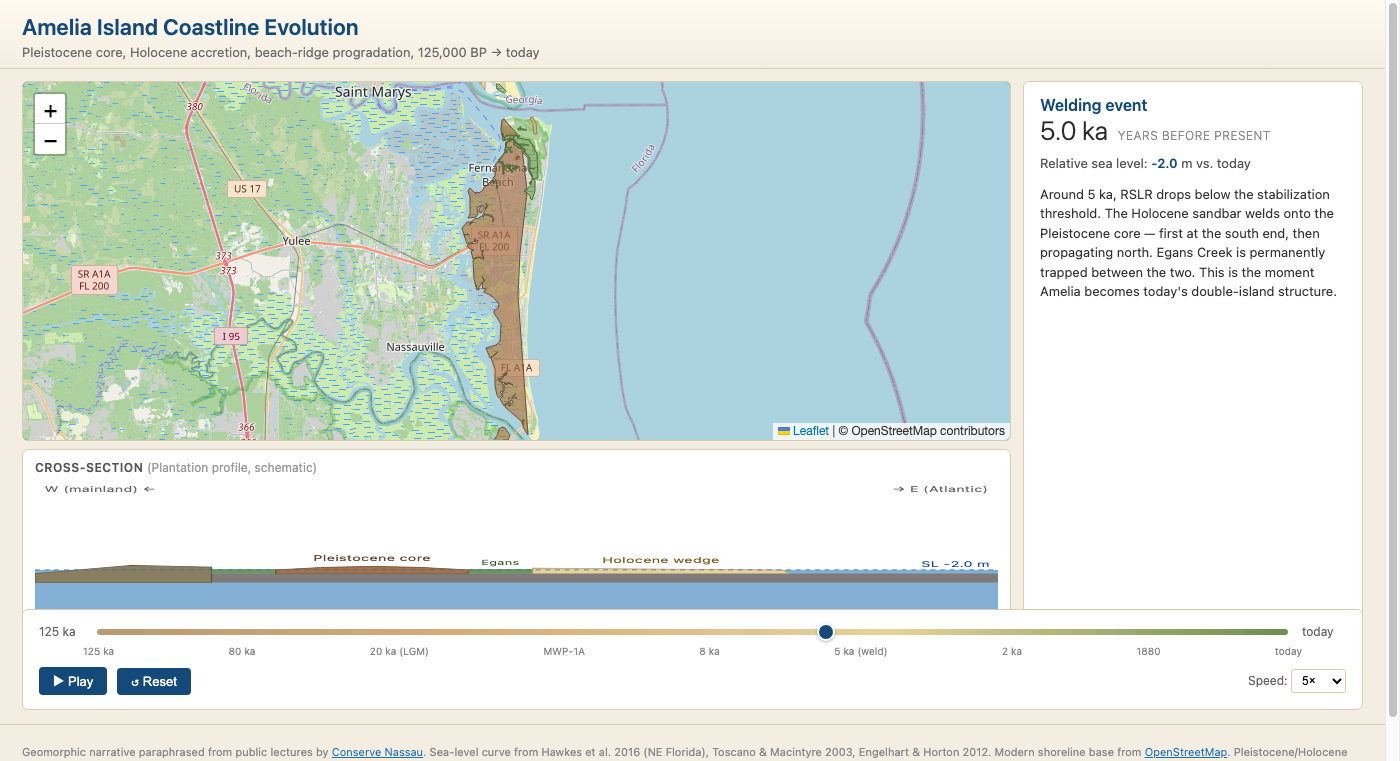
\includegraphics[width=0.95\textwidth]{fig/05_welding_5ka.png}
\caption{The welding event, 5\,ka. The Holocene sandbar has welded onto the
Pleistocene core. Egans Creek marsh is permanently trapped between them.
This is the visual climax of the simulation: the moment Amelia becomes today's
double-island.}
\label{fig:welding}
\end{figure}

\begin{figure}[h!]
\centering
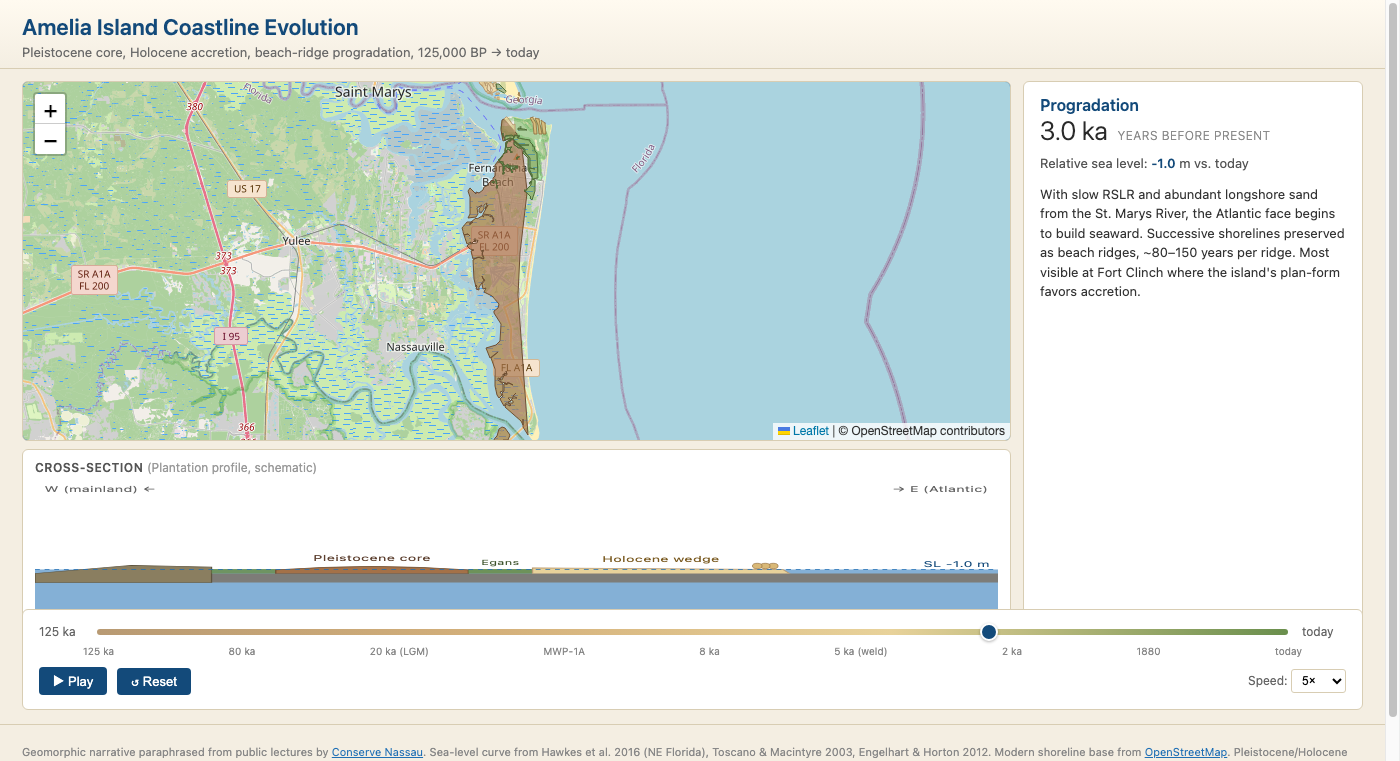
\includegraphics[width=0.95\textwidth]{fig/06_progradation_3ka.png}
\caption{Mid-Holocene progradation, 3\,ka. The Atlantic face begins
building seaward. Beach ridges appear as small arcs near Fort Clinch (north
end of the island). Sea level $-1$\,m; sea-level rise has dropped well
below the $\sim$2\,mm/yr stabilization threshold.}
\label{fig:progradation}
\end{figure}

\begin{figure}[h!]
\centering
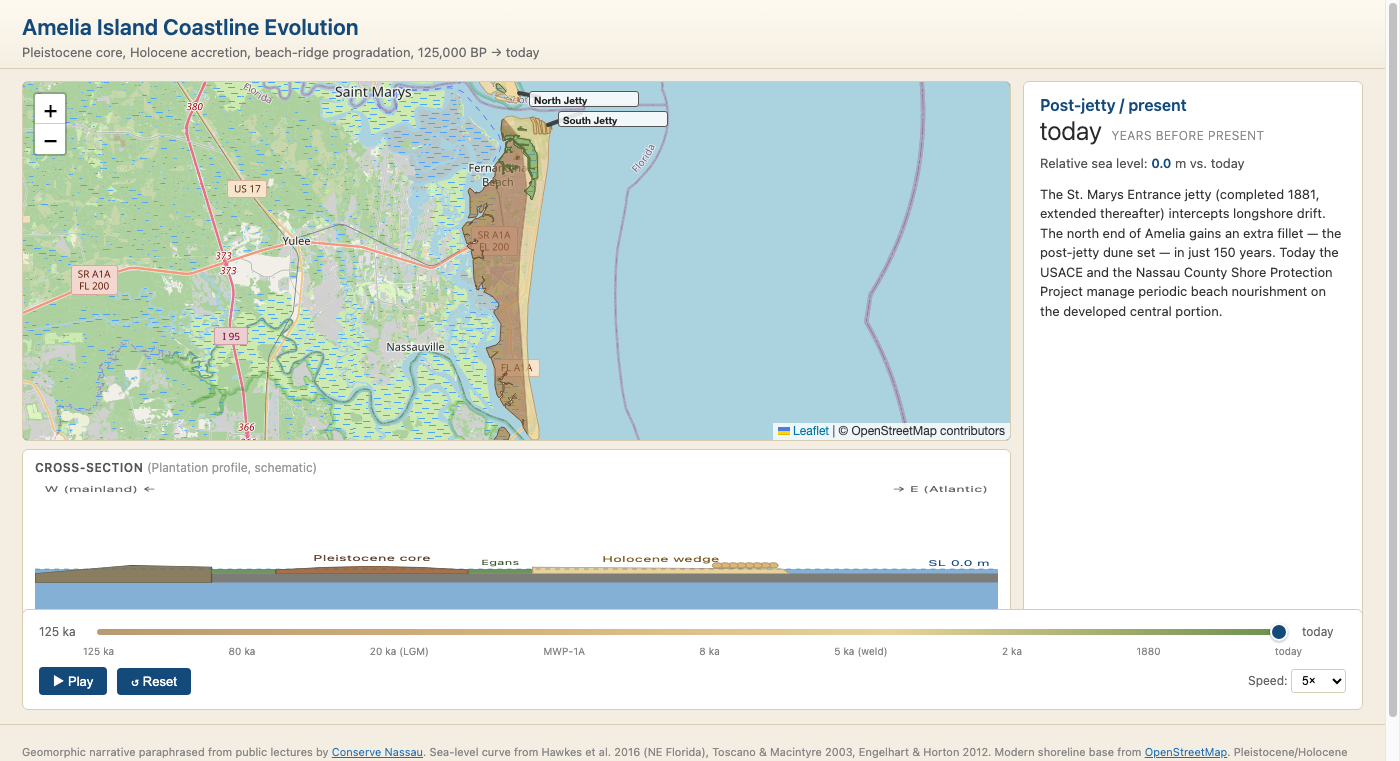
\includegraphics[width=0.95\textwidth]{fig/09_present.png}
\caption{Present, 2026\,CE. All eight modeled beach ridges are present at
Fort Clinch, including the post-jetty fillet added since 1881. The
cross-section shows the full ``two piles of sand on a bed of mud'' structure
that Frank Hopf emphasizes: Pleistocene core on the west, Egans Creek marsh in
the middle, Holocene wedge with beach ridges on the east.}
\label{fig:present}
\end{figure}

\begin{figure}[h!]
\centering
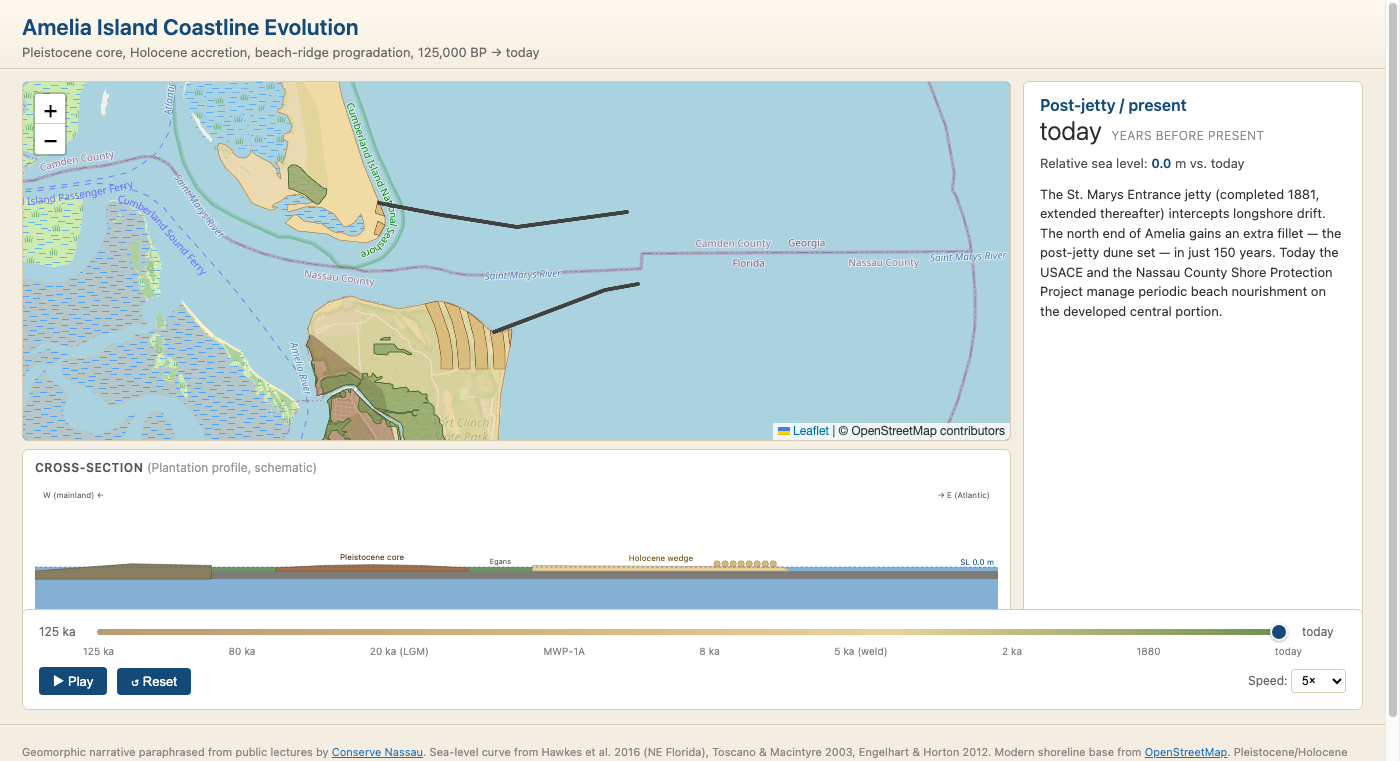
\includegraphics[width=0.95\textwidth]{fig/jetties_zoom.png}
\caption{Zoomed view of the St.\ Marys River Entrance jetties at present-day
(zoom 13). Both jetty geometries are pulled directly from NOAA Electronic
Navigational Chart US5FL8CE (SLCONS layer, CATSLC=4). The \textbf{North Jetty}
(upper line, Cumberland Island/Georgia side) is $\sim$4.14\,km long. The
\textbf{South Jetty} (lower line, Amelia/Fort Clinch/Florida side) is
$\sim$2.50\,km long. Both jetties were completed 1881--1893 by the US Army
Corps of Engineers to maintain the navigation channel into Cumberland Sound.
The ratio of approximately 1.65:1 (North:South) matches the surveyed
geometry on the nautical chart.}
\label{fig:jetties_zoom}
\end{figure}

\section{Reproducibility}

The figures above are not hand-curated. They are produced by running the
Selenium suite, which drives the viewer through every defined snapshot,
asserts that the expected layer kinds are rendered at each timestep, and
saves a screenshot per snapshot. To reproduce:

\begin{Verbatim}[fontsize=\small]
python3 -m venv venv
source venv/bin/activate
pip install selenium Pillow youtube-transcript-api yt-dlp
python scripts/fetch_osm.py
python scripts/build_snapshots.py
python tests/auto/test_viewer.py
pdflatex docs/geomorphological-experiments.tex
\end{Verbatim}

\noindent The Selenium suite exits with status 0 when all snapshots render
correctly. Failures are reported as ``FAIL'' lines and logged to
\texttt{tests/auto/test\_viewer.log}. The figures in
\texttt{docs/fig/} are overwritten each run, so this document always
reflects the current state of the viewer.

\section{Acknowledgements}

The geomorphic narrative summarized here draws extensively from a series of
public lectures given by \textbf{Dr.\ Frank Hopf, P.E.}\ (coastal
geomorphologist and professional engineer), presented through the
\href{https://www.youtube.com/@conservenassauflorida}{Conserve Nassau Florida}
organization \cite{cn_channel}. Three of those lectures provided the
narrative arc for the simulation:

\begin{itemize}[leftmargin=2em]
\item \emph{Hopf: A Fragile Barrier Island} (64 min) \cite{cn_hopf} ---
the master overview of formation, sea-level history, and present-day
fragility.
\item \emph{Dunes: Not Just a Pile of Sand --- Part 1: Pangaea to Present}
(28 min) \cite{cn_dunes1} --- the 400-million-year geologic context and
specific spatial references for Amelia's Pleistocene and Holocene history.
\item \emph{Dunes: Not Just a Pile of Sand --- Part 2: Our Holocene Dunes}
(33 min) \cite{cn_dunes2} --- Holocene dune development and the post-jetty
modifications since 1881.
\end{itemize}

\noindent A fourth source, the visual report \cite{cn_hopf_videoreport},
synthesizes Hopf's lectures via automated multimodal analysis of the
video frames (in addition to the spoken-word transcripts). This source
supplied the pedological terminology (Spodosols/Entisols, Bh horizon),
the dune-plant Latin names (\emph{Uniola paniculata},
\emph{Panicum amarum}, \emph{Ipomoea pes-caprae}), and the heavy-mineral
provenance (zircon, staurolite, tourmaline)---specifics that the
auto-captions of the spoken track did not reliably capture.

\noindent Transcripts were extracted programmatically from the YouTube
auto-captions, then mined for dates, distances, ridge-set descriptions, and
cross-section locations. Transcript material is paraphrased here under fair
use for non-commercial educational illustration. Direct quotations are
clearly marked. The original recordings remain the canonical source.

We also acknowledge the underlying peer-reviewed work that frames Amelia
Island's geomorphology, particularly Hawkes et al.\ \cite{hawkes2016} for the
NE Florida sea-level reconstruction, Hoyt and Hails \cite{hoyt1967} for the
Georgia Bight stratigraphic framework, and Mariotti \cite{mariotti2021} for
the modern process-based understanding of barrier-island stabilization.

\begin{thebibliography}{99}

\bibitem{hawkes2016}
Hawkes, A.~D., Kemp, A.~C., Donnelly, J.~P., Horton, B.~P., Peltier, W.~R.,
Cahill, N., et al.\ (2016).
Relative sea-level change in northeastern Florida (USA) during the last
$\sim$8.0\,ka.
\emph{Quaternary Science Reviews}, 142, 90--101.
\url{https://www2.whoi.edu/site/coastalgroup/wp-content/uploads/sites/139/2021/07/Hawkes-2016-Relative-sea-level-change-in-northeastern-Florida-USA-during-the-last-8.0-KA.pdf}

\bibitem{engelhart2012}
Engelhart, S.~E., and Horton, B.~P.\ (2012).
Holocene sea-level database for the Atlantic coast of the United States.
\emph{Quaternary Science Reviews}, 54, 12--25.

\bibitem{toscano2003}
Toscano, M.~A., and Macintyre, I.~G.\ (2003).
Corrected western Atlantic sea-level curve for the last 11{,}000 years based on
calibrated $^{14}$C dates from \emph{Acropora palmata} framework and intertidal
mangrove peat.
\emph{Coral Reefs}, 22, 257--270.

\bibitem{hoyt1967}
Hoyt, J.~H., and Hails, J.~R.\ (1967).
Pleistocene shoreline sediments in coastal Georgia: deposition and modification.
\emph{Science}, 155(3769), 1541--1543.
\url{https://www.science.org/doi/10.1126/science.155.3769.1541}

\bibitem{mariotti2021}
Mariotti, G.\ (2021).
Self-organization of coastal barrier systems during the Holocene.
\emph{Journal of Geophysical Research: Earth Surface}, 126.
\url{https://agupubs.onlinelibrary.wiley.com/doi/full/10.1029/2020JF005867}

\bibitem{georgiabight}
Hayes, M.~O.\ (1994).
The Georgia Bight Barrier System.
Chapter 7 in R.\,A.\ Davis Jr.\ (Ed.), \emph{Geology of Holocene Barrier
Island Systems}, pp.\ 233--304. Springer-Verlag, Berlin.
\url{https://link.springer.com/chapter/10.1007/978-3-642-78360-9_7}

\bibitem{georgyofflorida}
Wikipedia contributors.\ \emph{Geology of Florida}.
\url{https://en.wikipedia.org/wiki/Geology_of_Florida}

\bibitem{rink2008}
Rink, W.~J., and Forrest, B.\ (2005).
Dating evidence for the accretion history of beach ridges on Cape Canaveral and
Merritt Island, Florida, USA.
\emph{Journal of Coastal Research}, 21(5), 1000--1008.

\bibitem{forrest2007}
Forrest, B.~M., Rink, W.~J., et al.\ (2008).
New quartz OSL ages for beach ridges on the St.\ Vincent Island Holocene
strandplain, Florida, USA.
\emph{Journal of Coastal Research}, Special Issue 24(SP1).

\bibitem{cn_hopf}
Hopf, F.\ (Conserve Nassau Florida).
\emph{Hopf: A Fragile Barrier Island} [public lecture, video].
YouTube, May 2026 (accessed). 64 min.
\url{https://www.youtube.com/watch?v=SNysbbhGiDY}

\bibitem{cn_dunes1}
Hopf, F.\ (Conserve Nassau Florida).
\emph{Dunes: Not Just a Pile of Sand --- Part 1: Pangaea to Present} [public
lecture, video]. YouTube, accessed May 2026. 28 min.
\url{https://www.youtube.com/watch?v=nUIkpNE7k5E}

\bibitem{cn_dunes2}
Hopf, F.\ (Conserve Nassau Florida).
\emph{Dunes: Not Just a Pile of Sand --- Part 2: Our Holocene Dunes} [public
lecture, video]. YouTube, accessed May 2026. 33 min.
\url{https://www.youtube.com/watch?v=JvtDEisEI4c}

\bibitem{cn_channel}
Conserve Nassau Florida.\ YouTube channel.
\url{https://www.youtube.com/@conservenassauflorida}

\bibitem{cn_hopf_videoreport}
Hopf, F., P.E.\ \emph{Geomorphological Report: Amelia Island, Florida}
(synthesized from the lecture series ``Dunes: Not just a pile of sand''
via automated multimodal video analysis of the Conserve Nassau YouTube
recordings, May 2026).
\texttt{docs/hopf\_amelia\_island\_geomorphology\_report.md}.

\bibitem{leaflet}
Leaflet --- an open-source JavaScript library for mobile-friendly interactive
maps. \url{https://leafletjs.com}

\bibitem{selenium}
Selenium WebDriver. \url{https://www.selenium.dev}

\end{thebibliography}

\end{document}
